\section{Auswertung}
\label{sec:Auswertung}

Bei den Messgeräten Ohm-, Volt- und Amperemeter sowie für die Stoppuhr wird eine Messunsicherheit abgeschätzt:
\begin{align*}
	\sigma_R &= \SI{0.1}{\ohm}\\
	\sigma_U &= \SI{0.01}{\volt}\\
	\sigma_I &= \SI{0.1}{\milli\ampere}\\
	\sigma_{\symup\Delta t} &= \SI{0.1}{\second}	\,\text.
\end{align*}

\subsection{Messung der Molwärme}
Die Molwärme $C_V$ bei konstantem Volumen zu bestimmen, gestaltet sich experimentell schwierig. Einfacher ist es, zunächst die Molwärme $C_p$ bei konstantem Druck zu bestimmen und diese mittels Gleichung
\begin{equation}
  C_V = C_p - 9 \cdot \alpha^2 \cdot \kappa V_0 \cdot T
\end{equation}
umzurechnen.
Dabei bezeichnet $\kappa$ das Kompressionsmodul, $T$ die Temperatur, $V_0 = M/\rho$ das Molvolumen und \alpha den temperaturabhängigen Ausdehnungskoeffizient, der der Anleitung \cite{V47} entnommen wird.
Die Ergebisse sind in Tabelle \ref{tab:tab2} aufgeführt.
Die Molwärme $C_p$ kann mit der zugeführten elektrischen Energie bestimmt werden.
Diese kann aus den Werten in Tabelle \ref{tab:tab1} mit
\begin{align}
	E &= U \cdot I \cdot \symup{\Delta} t,\\
	C_p &= \frac{M}{m}\cdot\frac{E}{\symup{\Delta} T}
	\label{eqn:cp}
\end{align}
berechnet werden.
Dabei steht $E$ für die zugeführte Energie, $U$ für die Spannung, $I$ für die Stromstärke, $\symup\Delta t$ für das Zeitintervall, $\symup\Delta T$ für den Temperaturunterschied, $M$ für die molare Masse und $m$ für die Probenmasse.
In Tabelle \ref{tab:tab1} sind außer den bereits genannten Größen die berechneten Molwärmen eingetragen.
Alle materialspezifschen Konstanten werden der Quelle \cite{kupfer} entnommen.
\begin{align*}
  M &= \SI{0.0635}{\kilo\gram\mol^{-1}} \\
  \kappa &= \SI{137}{GPa} \\
  \rho &= \SI{8960}{\kilo\gram\meter^{-3}}
\end{align*}
Die Masse der Probe beträgt nach der Anleitung \cite{V47} $m = \SI{0.342}{\kilo\gram}$.
Die Messunsicherheiten werden über die Gaußsche Fehlerfortpflanzung mit den folgenden Formeln berechnet:
\begin{align*}
	\sigma_E &= \sqrt{I^{2} U^{2} \sigma_{{\symup\Delta T}}^{2} + I^{2} {\symup\Delta T}^{2} \sigma_{U}^{2} + U^{2} {\symup\Delta T}^{2} \sigma_{I}^{2}}\\
	\sigma_{C_p} &= \sqrt{\frac{E^{2} M^{2} \sigma_{{\symup\Delta T}}^{2}}{{\symup\Delta T}^{4} m^{2}} +\frac{M^{2} \sigma_{E}^{2}}{{\symup\Delta T}^{2} m^{2}}}\\
	\sigma_{C_V} &= \sqrt{324 T^{2} V_{0}^{2} \alpha^{2} \kappa^{2} \sigma_{\alpha}^{2} + 81 V_{0}^{2} \alpha^{4} \kappa^{2} \sigma_{T}^{2} + \sigma_{C_{p}}^{2}}\,\text.
\end{align*}

Zur Übersicht sind die Werte für $C_V$ und $C_p$ in Abbildung \ref{fig:cp} und \ref{fig:cv} in Abhängigkeit von der, über den Messwiderstand berechneten, Temperatur geplottet.
Die Einheiten für $C_V$ und $C_p$ wurden in den Tabellen aus Platzgründen bewusst weggelassen und werden hier seperat angegeben:
\begin{equation*}
	[C_V] = [C_p] = \si{\joule\per\mole\per\kelvin}\,\text.
\end{equation*}

\begin{figure}
	\centering
	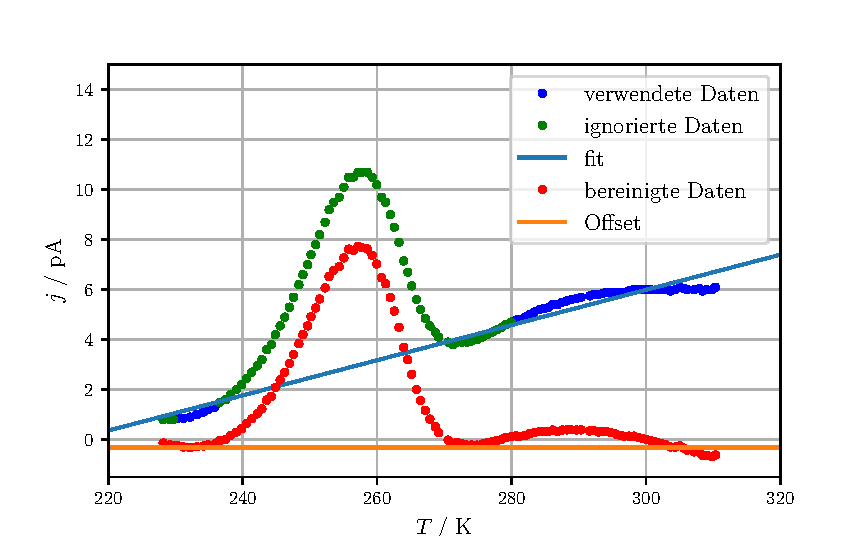
\includegraphics[width=\textwidth]{build/plot1.pdf}
	\caption{Die Molwärmen bei konstantem Druck in Abhängigkeit der Temperatur.}
	\label{fig:cp}
\end{figure}

\begin{figure}
	\centering
	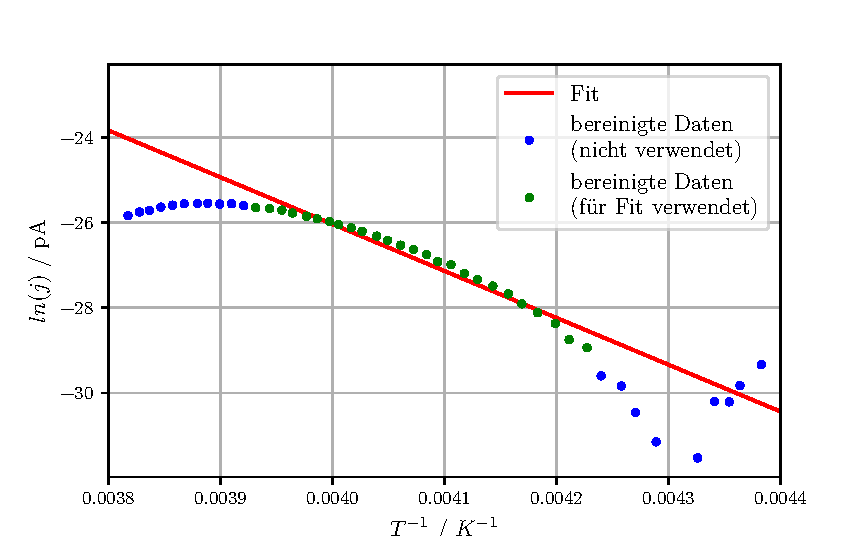
\includegraphics[width=\textwidth]{build/plot3.pdf}
	\caption{Die Molwärmen bei konstantem Volumen in Abhängigkeit der Temperatur.}
	\label{fig:cv}
\end{figure}

\begin{table}
  \centering
  \caption{Temperaturunterschied $\Delta T$ der Probe im Zeitintervall $\Delta t$, in dem die Spannung $U$ und die Stromstärke $I$ angelegt ist und resultierende Molwärme $C_p$.}
  \label{tab:tab1}
  \begin{tabular}{c c c c c}
    \toprule
		$\Delta T$/K & $U$/V & $I$/A & $\Delta t$/s & $C_p$ \\
    \midrule
		$6.14\pm0.33$ & $16.77\pm0.01$ & $0.1603\pm0.0001$ & $150\pm5$ & $12.2\pm0.8$ \\
		$4.97\pm0.33$ & $16.90\pm0.01$ & $0.1613\pm0.0001$ & $150\pm5$ & $15.3\pm1.1$ \\
		$4.51\pm0.34$ & $16.97\pm0.01$ & $0.1619\pm0.0001$ & $150\pm5$ & $17.0\pm1.4$ \\
		$4.52\pm0.34$ & $17.02\pm0.01$ & $0.1622\pm0.0001$ & $150\pm5$ & $17.0\pm1.4$ \\
		$4.29\pm0.34$ & $17.06\pm0.01$ & $0.1625\pm0.0001$ & $150\pm5$ & $18.0\pm1.5$ \\
		$4.06\pm0.34$ & $17.09\pm0.01$ & $0.1627\pm0.0001$ & $150\pm5$ & $19.1\pm1.7$ \\
		$4.30\pm0.34$ & $17.12\pm0.01$ & $0.1629\pm0.0001$ & $150\pm5$ & $18.0\pm1.5$ \\
		$4.31\pm0.34$ & $17.14\pm0.01$ & $0.1630\pm0.0001$ & $150\pm5$ & $18.0\pm1.5$ \\
		$4.32\pm0.34$ & $17.16\pm0.01$ & $0.1631\pm0.0001$ & $150\pm5$ & $18.0\pm1.5$ \\
		$3.85\pm0.34$ & $17.17\pm0.01$ & $0.1632\pm0.0001$ & $150\pm5$ & $20.3\pm1.9$ \\
		$3.85\pm0.34$ & $17.20\pm0.01$ & $0.1634\pm0.0001$ & $150\pm5$ & $20.3\pm1.9$ \\
		$3.86\pm0.34$ & $17.21\pm0.01$ & $0.1635\pm0.0001$ & $150\pm5$ & $20.3\pm1.9$ \\
		$3.87\pm0.34$ & $17.24\pm0.01$ & $0.1635\pm0.0001$ & $150\pm5$ & $20.3\pm1.9$ \\
		$3.88\pm0.34$ & $17.24\pm0.01$ & $0.1636\pm0.0001$ & $150\pm5$ & $20.3\pm1.9$ \\
		$3.88\pm0.34$ & $17.25\pm0.01$ & $0.1636\pm0.0001$ & $150\pm5$ & $20.2\pm1.9$ \\
		$3.65\pm0.34$ & $17.26\pm0.01$ & $0.1636\pm0.0001$ & $150\pm5$ & $21.6\pm2.2$ \\
		$3.65\pm0.34$ & $17.27\pm0.01$ & $0.1637\pm0.0001$ & $150\pm5$ & $21.6\pm2.2$ \\
		$3.66\pm0.34$ & $17.27\pm0.01$ & $0.1638\pm0.0001$ & $150\pm5$ & $21.5\pm2.2$ \\
		$3.42\pm0.35$ & $17.28\pm0.01$ & $0.1638\pm0.0001$ & $150\pm5$ & $23.1\pm2.5$ \\
		$3.67\pm0.35$ & $17.29\pm0.01$ & $0.1638\pm0.0001$ & $150\pm5$ & $21.5\pm2.1$ \\
		$3.68\pm0.35$ & $17.30\pm0.01$ & $0.1639\pm0.0001$ & $150\pm5$ & $21.5\pm2.1$ \\
		$3.68\pm0.35$ & $17.30\pm0.01$ & $0.1639\pm0.0001$ & $150\pm5$ & $21.4\pm2.1$ \\
		$3.69\pm0.35$ & $17.31\pm0.01$ & $0.1640\pm0.0001$ & $150\pm5$ & $21.4\pm2.1$ \\
		$8.13\pm0.35$ & $17.32\pm0.01$ & $0.1641\pm0.0001$ & $300\pm5$ & $21.3\pm1.1$ \\
		$7.42\pm0.35$ & $17.33\pm0.01$ & $0.1641\pm0.0001$ & $300\pm5$ & $22.8\pm1.2$ \\
		$6.95\pm0.35$ & $17.33\pm0.01$ & $0.1641\pm0.0001$ & $300\pm5$ & $21.9\pm1.1$ \\
		$7.22\pm0.35$ & $17.34\pm0.01$ & $0.1642\pm0.0001$ & $300\pm5$ & $23.5\pm1.3$ \\
		$6.74\pm0.35$ & $17.34\pm0.01$ & $0.1642\pm0.0001$ & $300\pm5$ & $22.6\pm1.2$ \\
		$7.01\pm0.35$ & $17.34\pm0.01$ & $0.1642\pm0.0001$ & $300\pm5$ & $24.3\pm1.4$ \\
		$6.5\pm0.4$   & $17.34\pm0.01$ & $0.1642\pm0.0001$ & $300\pm5$ & $25.2\pm1.5$ \\
		$6.3\pm0.4$   & $17.35\pm0.01$ & $0.1643\pm0.0001$ & $300\pm5$ & $25.2\pm1.5$ \\
		$6.3\pm0.4$   & $17.34\pm0.01$ & $0.1643\pm0.0001$ & $300\pm5$ & $25.1\pm1.5$ \\
		$6.3\pm0.4$   & $17.34\pm0.01$ & $0.1643\pm0.0001$ & $300\pm5$ & $18.9\pm0.9$ \\
		$8.4\pm0.4$   & $17.34\pm0.01$ & $0.1643\pm0.0001$ & $300\pm5$ & $20.1\pm1.0$ \\
		$7.9\pm0.4$   & $17.34\pm0.01$ & $0.1644\pm0.0001$ & $300\pm5$ & $25.9\pm1.6$ \\
		$6.1\pm0.4$   & $17.34\pm0.01$ & $0.1644\pm0.0001$ & $300\pm5$ & $24.8\pm1.5$ \\
		$6.4\pm0.4$   & $17.34\pm0.01$ & $0.1644\pm0.0001$ & $300\pm5$ & $25.8\pm1.6$ \\
		$6.2\pm0.4$   & $17.33\pm0.01$ & $0.1644\pm0.0001$ & $300\pm5$ & $25.7\pm1.6$ \\
		$6.2\pm0.4$   & $17.33\pm0.01$ & $0.1644\pm0.0001$ & $300\pm5$ & $24.6\pm1.5$ \\

    \bottomrule
  \end{tabular}
\end{table}

\begin{table}
  \centering
  \caption{Die Molwärme $C_p$, die Temperatur $T$, der temperaturabhängige Ausdehnungskoeffizient $\alpha$ und die daraus resultierende Molwärme $C_V$.}
  \label{tab:tab2}
  \begin{tabular}{c c c c}
    \toprule
		$T$/K & $C_p$ & $\alpha$/K & $C_V$ \\
    \midrule
		$82.47\pm0.24$  & $12.2\pm0.8$ & $\num{8.693(22)e-6}$ & $12.1+/-0.8$ \\
		$88.60\pm0.24$  & $15.3\pm1.1$ & $\num{9.260(22)e-6}$ & $15.2+/-1.1$ \\
		$93.57\pm0.24$  & $17.0\pm1.4$ & $\num{9.720(22)e-6}$ & $16.9+/-1.4$ \\
		$98.08\pm0.24$  & $17.0\pm1.4$ & $\num{1.0137(22)e-5}$ & $16.9\pm1.4$ \\
		$102.59\pm0.24$ & $18.0\pm1.5$ & $\num{1.0554(22)e-5}$ & $17.9\pm1.5$ \\
		$106.88\pm0.24$ & $19.1\pm1.7$ & $\num{1.0951(22)e-5}$ & $19.0\pm1.7$ \\
		$110.94\pm0.24$ & $18.0\pm1.5$ & $\num{1.1326(22)e-5}$ & $17.9\pm1.5$ \\
		$115.24\pm0.24$ & $18.0\pm1.5$ & $\num{1.1724(22)e-5}$ & $17.9\pm1.5$ \\
		$119.55\pm0.24$ & $18.0\pm1.5$ & $\num{1.2123(22)e-5}$ & $17.9\pm1.5$ \\
		$123.87\pm0.24$ & $20.3\pm1.9$ & $\num{1.2523(22)e-5}$ & $20.1\pm1.9$ \\
		$127.72\pm0.24$ & $20.3\pm1.9$ & $\num{1.2879(22)e-5}$ & $20.1\pm1.9$ \\
		$131.58\pm0.24$ & $20.3\pm1.9$ & $\num{1.3235(22)e-5}$ & $20.1\pm1.9$ \\
		$135.44\pm0.24$ & $20.3\pm1.9$ & $\num{1.3465(5)e-5}$ & $20.1\pm1.9$ \\
		$139.31\pm0.24$ & $20.3\pm1.9$ & $\num{1.3545(5)e-5}$ & $20.0\pm1.9$ \\
		$143.18\pm0.24$ & $20.2\pm1.9$ & $\num{1.3626(5)e-5}$ & $20.0\pm1.9$ \\
		$147.07\pm0.24$ & $21.6\pm2.2$ & $\num{1.3707(5)e-5}$ & $21.3\pm2.2$ \\
		$150.71\pm0.24$ & $21.6\pm2.2$ & $\num{1.3783(5)e-5}$ & $21.3\pm2.2$ \\
		$154.36\pm0.24$ & $21.5\pm2.2$ & $\num{1.3859(5)e-5}$ & $21.3\pm2.2$ \\
		$158.02\pm0.24$ & $23.1\pm2.5$ & $\num{1.3935(5)e-5}$ & $22.8\pm2.5$ \\
		$161.44\pm0.24$ & $21.5\pm2.1$ & $\num{1.4006(5)e-5}$ & $21.2\pm2.1$ \\
		$165.11\pm0.24$ & $21.5\pm2.1$ & $\num{1.4082(5)e-5}$ & $21.2\pm2.1$ \\
		$168.79\pm0.25$ & $21.4\pm2.1$ & $\num{1.4158(5)e-5}$ & $21.2\pm2.1$ \\
		$172.47\pm0.25$ & $21.4\pm2.1$ & $\num{1.4235(5)e-5}$ & $21.1\pm2.1$ \\
		$184.29\pm0.25$ & $21.3\pm1.1$ & $\num{1.4481(5)e-5}$ & $21.0\pm1.1$ \\
		$191.71\pm0.25$ & $22.8\pm1.2$ & $\num{1.4635(5)e-5}$ & $22.4\pm1.2$ \\
		$198.66\pm0.25$ & $21.9\pm1.1$ & $\num{1.4780(5)e-5}$ & $21.6\pm1.1$ \\
		$205.88\pm0.25$ & $23.5\pm1.3$ & $\num{1.4930(5)e-5}$ & $23.1\pm1.3$ \\
		$212.62\pm0.25$ & $22.6\pm1.2$ & $\num{1.5070(5)e-5}$ & $22.2\pm1.2$ \\
		$219.63\pm0.25$ & $24.3\pm1.4$ & $\num{1.5216(5)e-5}$ & $23.8\pm1.4$ \\
		$226.15\pm0.25$ & $25.2\pm1.5$ & $\num{1.5352(5)e-5}$ & $24.7\pm1.5$ \\
		$232.45\pm0.25$ & $25.2\pm1.5$ & $\num{1.5482(5)e-5}$ & $24.7\pm1.5$ \\
		$238.76\pm0.25$ & $25.1\pm1.5$ & $\num{1.5614(5)e-5}$ & $24.6\pm1.5$ \\
		$245.09\pm0.25$ & $18.9\pm0.9$ & $\num{1.5745(5)e-5}$ & $18.4\pm0.9$ \\
		$253.47\pm0.25$ & $20.1\pm1.0$ & $\num{1.5920(5)e-5}$ & $19.5\pm1.0$ \\
		$261.36\pm0.26$ & $25.9\pm1.6$ & $\num{1.6084(5)e-5}$ & $25.3\pm1.6$ \\
		$267.50\pm0.26$ & $24.8\pm1.5$ & $\num{1.6211(5)e-5}$ & $24.2\pm1.5$ \\
		$273.90\pm0.26$ & $25.8\pm1.6$ & $\num{1.6344(5)e-5}$ & $25.1\pm1.6$ \\
		$280.06\pm0.26$ & $25.7\pm1.6$ & $\num{1.6473(5)e-5}$ & $25.0\pm1.6$ \\
		$286.24\pm0.26$ & $24.6\pm1.5$ & $\num{1.6601(5)e-5}$ & $23.9\pm1.4$ \\
    \bottomrule
  \end{tabular}
\end{table}

\subsection{Experimentelle Bestimmung der Debye-Temperatur}

Zur Bestimmung der Debye-Temperatur werden die Molwärmen $C_V$ unter \SI{170}{\kelvin} betrachtet.
Die Quotienten $\theta_D / T$ können dann für ein gegebenes $C_V$ aus der Debye-Funktion aus der Anleitung \cite{V47} ausgelesen werden.
Die Werte dazu sind in der Tabelle \ref{tab:tab3} dargestellt.
Durch einfache Multiplikation kann dann die Debye-Temperatur bestimmt werden.

\begin{table}
  \centering
  \caption{Die Molwärme $C_v$, der Quotient $\theta_D / T$, die Temperatur $T$ und die resultierende Debye-Temperatur $\theta_D$.}
  \label{tab:tab3}
  \begin{tabular}{c c c c}
    \toprule
		$C_V$ & $\theta_D / T$ & $T$/K & $\theta_D$/ \\
    \midrule
		$12.1\pm0.8$ & $4.1$ & $ 82.47\pm0.24$ & $338.1\pm1.0$ \\
		$15.2\pm1.1$ & $3.3$ & $ 88.60\pm0.24$ & $292.4\pm0.8$ \\
		$16.9\pm1.4$ & $2.9$ & $ 93.57\pm0.24$ & $271.4\pm0.7$ \\
		$16.9\pm1.4$ & $2.9$ & $ 98.08\pm0.24$ & $284.4\pm0.7$ \\
		$17.9\pm1.5$ & $2.7$ & $102.59\pm0.24$ & $277.0\pm0.6$ \\
		$19.0\pm1.7$ & $2.4$ & $106.88\pm0.24$ & $256.5\pm0.6$ \\
		$17.9\pm1.5$ & $2.7$ & $110.94\pm0.24$ & $299.5\pm0.6$ \\
		$17.9\pm1.5$ & $2.7$ & $115.24\pm0.24$ & $311.1\pm0.6$ \\
		$17.9\pm1.5$ & $2.7$ & $119.55\pm0.24$ & $322.8\pm0.6$ \\
		$20.1\pm1.9$ & $2.1$ & $123.87\pm0.24$ & $260.1\pm0.5$ \\
		$20.1\pm1.9$ & $2.1$ & $127.72\pm0.24$ & $268.2\pm0.5$ \\
		$20.1\pm1.9$ & $2.1$ & $131.58\pm0.24$ & $276.3\pm0.5$ \\
		$20.1\pm1.9$ & $2.1$ & $135.44\pm0.24$ & $284.4\pm0.5$ \\
		$20.0\pm1.9$ & $2.2$ & $139.31\pm0.24$ & $306.5\pm0.5$ \\
		$20.0\pm1.9$ & $2.2$ & $143.18\pm0.24$ & $315.0\pm0.5$ \\
		$21.3\pm2.2$ & $1.8$ & $147.07\pm0.24$ & $264.7\pm0.4$ \\
		$21.3\pm2.2$ & $1.8$ & $150.71\pm0.24$ & $271.3\pm0.4$ \\
		$21.3\pm2.2$ & $1.8$ & $154.36\pm0.24$ & $277.9\pm0.4$ \\
		$22.8\pm2.5$ & $1.3$ & $158.02\pm0.24$ & $205.4\pm0.3$ \\
		$21.2\pm2.1$ & $1.8$ & $161.44\pm0.24$ & $290.6\pm0.4$ \\
		$21.2\pm2.1$ & $1.8$ & $165.11\pm0.24$ & $297.2\pm0.4$ \\
		$21.2\pm2.1$ & $1.8$ & $168.79\pm0.25$ & $303.8\pm0.4$ \\

    \bottomrule
  \end{tabular}
\end{table}

\subsection{Theoretische Bestimmung der Debye-Temperatur}

Aus der Gleichung (7) lässt sich die Debye-Frequenz berechnen.
Zuerst müssen aber die Größen $L^3$ und $N_L$ bestimmt werden.
Die Geschwindigkeiten $v_l$ und $v_{tr}$ sind aus der Anleitung \cite{V47} durch \SI{4.7}{\kilo\meter\second^{-1}}
und \SI{2.26}{\kilo\meter\second^{-1}} gegeben.
Die Teilchenzahl lässt sich durch den Zusammenhang
\begin{equation}
  N_L = \frac{m}{M} \cdot N_A
\end{equation}
berechnen.
Das Volumen $L^3$ kann bestimmt werden durch:
\begin{equation}
  L^3 = V = V_0 \cdot \frac{m}{M}
\end{equation}
Schlussendlich folgt die Debye-Frequenz mit $\omega_D = \SI{43e12}{Hz}$.
Daraus lässt sich mit der Gleichung
\begin{equation}
  \theta_D = \hbar \cdot \omega_D
\end{equation}
die Debye-Temperatur $\theta_D = \SI{332.48}{\kelvin}$ bestimmen.
